\documentclass[12pt,a4paper]{article}

\title{P-unit model by Henriette Walz \& Alexander Ott}
\author{Alexandra Rudnaya, Jan Grewe, Jan Benda}
\date{June 2022}

%%%%% layout %%%%%%%%%%%%%%%%%%%%%%%%%%%%%%%%%%%%%%%%%%%%%%%%%%%%%%%%%%%%%%%%
\usepackage[left=20mm,right=20mm,top=20mm,bottom=20mm]{geometry}
%\setcounter{secnumdepth}{-1}

%%%%% units %%%%%%%%%%%%%%%%%%%%%%%%%%%%%%%%%%%%%%%%%%%%%%%%%%%%%%%%%%%%%%%%%
\usepackage[mediumspace,mediumqspace,Gray,amssymb]{SIunits}      % \ohm, \micro

%%%%% math %%%%%%%%%%%%%%%%%%%%%%%%%%%%%%%%%%%%%%%%%%%%%%%%%%%
\usepackage{textcomp}
\usepackage{array}
\usepackage{amsmath}
\usepackage{amssymb}
\usepackage{graphicx}

%%%%% equation references %%%%%%%%%%%%%%%%%%%%%%%%%%%%%%%%%%%%%%%%%%%%%%%%%%%
\renewcommand{\eqref}[1]{(\ref{#1})}
\newcommand{\eqn}{Eq.}
\newcommand{\Eqn}{Eq.}
\newcommand{\eqns}{Eqs.}
\newcommand{\Eqns}{Eqs.}
\newcommand{\eqnref}[1]{\eqn~\eqref{#1}}
\newcommand{\Eqnref}[1]{\Eqn~\eqref{#1}}
\newcommand{\eqnsref}[1]{\eqns~\eqref{#1}}
\newcommand{\Eqnsref}[1]{\Eqns~\eqref{#1}}
 
%%%%% hyperef %%%%%%%%%%%%%%%%%%%%%%%%%%%%%%%%%%%%%%%%%%%%%%%%%%%%%%%%%%%%%%%
\usepackage{xcolor}
\usepackage[breaklinks=true,colorlinks=true,citecolor=blue!30!black,urlcolor=blue!30!black,linkcolor=blue!30!black]{hyperref}

%%%%% notes %%%%%%%%%%%%%%%%%%%%%%%%%%%%%%%%%%%%%%%%%%%%%%%%%%%%%%%%%%%%%%%%
\newcommand{\note}[2][]{\textbf{[#1: #2]}}

%%%%%%%%%%%%%%%%%%%%%%%%%%%%%%%%%%%%%%%%%%%%%%%%%%%%%%%%%%%%%%%%%%%%%%%%%%%%%
%%%%%%%%%%%%%%%%%%%%%%%%%%%%%%%%%%%%%%%%%%%%%%%%%%%%%%%%%%%%%%%%%%%%%%%%%%%%%
\begin{document}

\maketitle


\section{The model}

The input into the P-unit model, $x(t)$, is
\begin{itemize}
\item the fish's own EOD
  \begin{equation}
    \label{eod}
    x(t) = x_{EOD}(t) = \cos(2\pi f_{EOD} t)
  \end{equation}
  with EOD frequency $f_{EOD}$ and amplitude normalized to one.
\item the EOD multiplied with an amplitude modulation $AM(t)$:
  \begin{equation}
    \label{am}
    x(t) = (1+AM(t)) \cos(2\pi f_{EOD} t)
  \end{equation}
  For a random amplitude modulaten ($AM(t) = RAM(t)$) random numbers
  are drawn for each frequency up to $f_{EOD}/2$ in Fourier
  space. After backtransformation the resulting signal is scaled to
  the desired standard deviation relative to the EOD carrier.
\item a superposition of two EODs
  \begin{equation}
    \label{beat}
    x(t) = x_{EOD}(t) + x_{EOD1}(t) = \cos(2\pi f_{EOD} t) + \alpha_1 \cos(2\pi f_{EOD1} t)
  \end{equation}
  with the EOD of the second fish having frequency $f_{EOD1}$ and amplitude $\alpha_1$ relative to the amplitude of the receiving fish.
\item a superposition of many EODs
  \begin{equation}
    \label{multibeat}
    x(t) = x_{EOD}(t) + \sum_{i=1}^{n} x_{EODi}(t) = \cos(2\pi f_{EOD} t) + \sum_{i=1}^{n} \alpha_i \cos(2\pi f_{EODi} t) \; .
  \end{equation}
  For $n=2$ this is our cocktail-party problem.  
\end{itemize}
The input $x(t)$ is a normalized EOD and thus is unitless.

First, the input $x(t)$, is thresholded potentially at the synapse between the receptor cells and the afferent, and then low-pass filtered  with time constant $\tau_{d}$ by the afferent's dendrite:
\begin{equation}
  \label{dendrite}
  \tau_{d} \frac{d V_{d}}{d t} = -V_{d}+  \lfloor x(t) \rfloor_{0}^{p}
\end{equation}
Because the input is unitless, the dendritic voltage is unitless, too. $\lfloor x(t) \rfloor_{0}$ denotes the threshold operation that sets negative values to zero:
\begin{equation}
  \label{threshold}
  \lfloor x(t) \rfloor_0 = \left\{ \begin{array}{rcl} x(t) & ; & x(t) \ge 0 \\ 0 & ; & x(t) < 0 \end{array} \right.
\end{equation}
Usually the exponent $p$ is set to one (pure threshold). In our advanced models $p$ is set to three in order to reproduce responses to beats with difference frequencies above half of the EOD frequency.

This thresholding and low-pass filtering extracts the amplitude modulation of the input $x(t)$. The dendritic voltage $V_d(t)$ is the input to a leaky integrate-and-fire (LIF) model
\begin{equation}
  \label{LIF}
  \tau_{m} \frac{d V_{m}}{d t}  = - V_{m} + \mu + \alpha V_{d} - A + \sqrt{2D}\xi(t)
\end{equation}
where $\tau_{m}$ the membrane time constant, $\mu$ a fixed bias current, $\alpha$ a scaling factor for $V_{d}$, and $\sqrt{2D}\xi(t)$ a white noise of strength $D$. All terms in the LIF are unitless.

The adaptation current $A$ follows
\begin{equation}
  \label{adaptation}
  \tau_{A} \frac{d A}{d t} = - A
\end{equation}
with adaptation time constant $\tau_A$.

Whenever the membrane voltage $V_m(t)$ crosses the threshold $\theta=1$ a spike is generated, $V_{m}(t)$ is reset to $0$, the adaptation current is incremented by $\Delta A$, and integration of $V_m(t)$ is paused for the duration of a refractory period $t_{ref}$:
\begin{equation}
  \label{spikethresh}
  V_m(t) \ge \theta \; : \left\{ \begin{array}{rcl} V_m & \mapsto & 0 \\ A  & \mapsto & A + \Delta A/\tau_A \end{array} \right.
\end{equation}


\section{Parameter values}

\note[JB]{Sascha, list all parameters (table or itemize) plus time step of the model with typical values and the right (time) units}


\begin{table}[h!]
  \begin{center}
    \caption{Model parameters.}
    \label{tab:table1}
    \begin{tabular}{l|c|l}
      
      parameter & explanation & median parameter \\
      \hline
      $\alpha$  & stimulus scaling factor &  90.533695\\
      $\tau_{m}$  & membrane time constant &  0.001847\,s\\       
      $\mu$  & bias current &  -17.1875\\      
      $\sqrt{2D}$  & noise strength &  0.01848 \\      
      $\tau_{A}$  & adaption time constant &  0.111759\,s\\      
      $\Delta A$  & adaption strength &  0.122197\\      
      $\tau_{d}$  & time constant of dendritic low-pass filter &  0.002463\,s\\      
      $t_{ref}$  & absolute refractory period &  0.000965\,s\\     
	  $\Delta t$  & time step &  0.00005\,s\\           
    \end{tabular}
  \end{center}
\end{table}
\begin{figure*}[tp]
  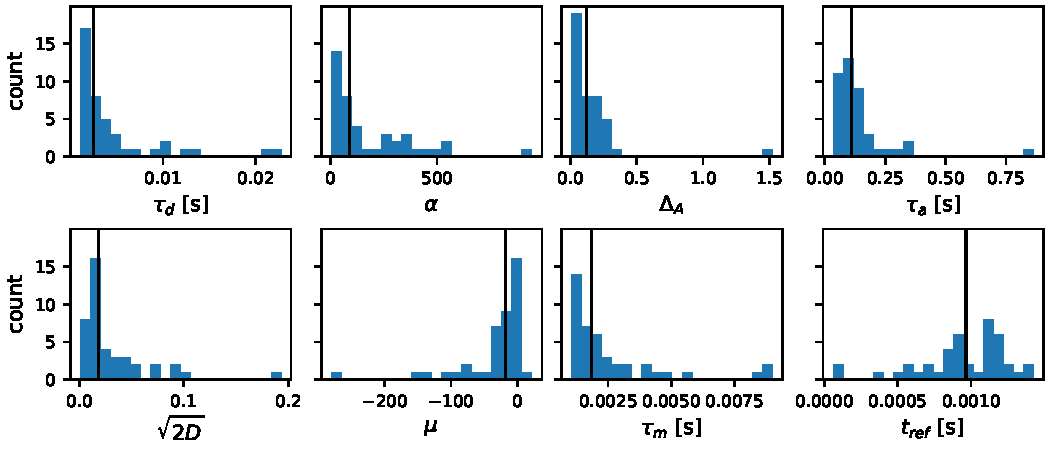
\includegraphics{parameter_distribution}
  \caption{\label{parameter_distribution} The distribution of the model parameters.
}
\end{figure*}





\section{Numerical implementation}




\note[JB]{Sascha: This is Alexander Ott's code from the git repository, right?}
\note[SR]{Yes that is correct.}
The ODEs are integrated by the Euler forward method with time-step $\Delta t$.

For the intrinsic noise of the model $\xi(t)$ in each time step $i$ a random number is drawn from a normal distribution $\mathcal{N}(0,\,1)$ with zero mean and standard deviation of one. This number is multiplied with $\sqrt{2D}$ and divided by $\sqrt{\Delta t}$:
\begin{equation}
  \label{LIFintegration}
  V_{m_{i+1}}  = V_{m_i} + \left(-V_{m_i} + \mu + \alpha V_{d_i} - A_i + \sqrt{\frac{2D}{\Delta t}}\mathcal{N}(0,\,1)_i\right) \frac{\Delta t}{\tau_m}
\end{equation}
\note[JB]{Benjamin: wir haben das Rauschen innerhalb der Klammer. Damit ist zwar das $\sqrt{\Delta t}$ richtig, aber wir teilen noch durch $\tau_m$. Damit sind effektiv unsere $D$ Werte andere als wenn wir den Rauschterm ausserhalb der Klammer haetten (so machst du das glaube ich immer).}

The noise strength values from the table in fact equal $\sqrt{2D}$ and not $D$.



\note[JB]{we need to clean up that noise issue}
\note[SR]{D in Tabelle angepasst, D im Code angepasst, nnoise mal Wurzel dt auch machen?}



\section{Cell Characteristics}
The cells were characterized by ten parameters: 6 for the baseline (mean firing rate, coefficient of variation (CV), vector strength (VS), serial correlation, the interspike interval (ISI) histogram, burstiness of the ISI) and 4 for the f-I curve (the detections of $f_{0}$ and $f_{\inf}$ responses for each contrast, the slope of the linear fit into the $f_{\inf}$ and the frequency trace of one
step response of $f_{0}$). These parameters will be described in the following paragraphs.


For the baseline the mean firing rate was calculated by dividing the number of spikes in the recording by the recording time.

The coefficient of variation
\begin{equation}
  \label{CV}
  CV = \frac{STD(ISI)}{\langle ISI \rangle}.
\end{equation}
is defined as the standard deviation (STD) of the interspike intervals ($ISI$) divided by the mean ISI.

The vector strength is a measure of how strong the cell locks to a phase of the EOD. It was calculated, by placing each spike on a unit circle depending on the relative spike time $t_{i}$ of how much time has passed since the start of
the current EOD period in relation to the EOD period length. This set of vectors is then averaged and the absolute value of this average vector describes the VS. If the VS is zero the spikes happen equally in all phases of the EOD while if it is one all spikes happen at the exact same phase of the EOD.
\begin{equation}
  \label{vs}
  vs = |\frac{1}{n} \sum_n e^{i\omega t_{i}}|.
\end{equation}

The serial correlation with lag k (SCk) of $T$ is a measure how the ISI $T_{i}$ (the i-th ISI) influences the $T_{i+k}$ the ISI with a lag of k intervals.

The ISI-histogram was calculated within a range of 0--50 \,ms and a bin size of 0.1\,ms. The burstiness was calculated as the percentage of ISI smaller than 2.5 EOD periods multiplied by the average ISI. This gives a rough measure of how often a cell fires in the immediately following EOD periods compared to its average firing frequency.

P-units react to a step in EOD amplitude with a strong onset response decaying back to a steady state response. This
adaption behavior of the cell was characterized by the f-I curve measurements. First the ISI frequency trace for each stimulus was calculated. The ISI frequency of a time point $t$ is defined as $\frac{1}{T_{i}}$ with $T_{i}$ the ISI the time point t falls into. This gives a frequency trace
starting with the first spike and ending at the last spike. For further analysis, all trials of a specific contrast were averaged over the trials with the resolution of the sampling rate. This results in a trial-averaged step response for each contrast. In this firing frequency trace the baseline frequency, the onset $f_{0}$ and steady-state $f_{\inf}$ response were detected. The baseline frequency was measured as the mean of the firing frequency 25\,ms after recording start up to 25\,ms before the stimulus start. $f_{0}$ was then defined as the largest deviation from the baseline frequency, within the first 25\,ms after
stimulus onset. If there was no deviation farther than the minimum or maximum before the stimulus start, then the average frequency in that 25\,ms time window was used. This
approximation made the detection of $f_{0}$ more stable for small contrasts and trials with high variation in their firing rates. The $f_{\inf}$ response was estimated as the average firing frequency in the 100\,ms time window ending 25\,ms before the end of the stimulus. Afterwards a Boltzmann function was fitted to the onset response and a rectified line:
\begin{equation}
  \label{f_inf}
  f_{\inf}(I) = \lfloor mI+c \rfloor_0.
\end{equation}
was fitted to the steady-state responses.


\end{document}
